\chapter[Desarrollo]{\label{ch:desarrollo}Desarrollo}

\section{\label{sec:des-intro}Introducción}

A partir de todos los puntos mencionados en el capitulo \ref{ch:marco-teorico} y dadas cada una de las características se optó por el \textit{Lenguaje de programación C} debido a ser un lenguaje de nivel medio que permite acceder a direcciones de memoria como un lenguaje de bajo nivel y además de su sintaxis ser conocida como de alto nivel, esto lo hace un lenguaje más potente  en esta línea, también cabe destacar que el lenguaje de programación C es un lenguaje compilado, esto permite que no se necesita utilizar de una maquina virtual o un interprete para procesar sus ejecuciones o el código fuente como lo realizan otros lenguajes, con esto solo se debe compilar una vez y ejecutar el código iterativamente. En términos de tiempos de ejecución de instrucciones como se aprecia en la gráfica de la figura \ref{speed}, se aprecia que el lenguaje de programación C es más veloz que muchos otros lenguajes, debido a las características ya mencionadas.\\
Ya acotando el rango de lenguajes entre C, C++, Python como se aprecia en la gráfica \ref{speedheap}, el lenguaje de programación C es considerablemente más veloz para procesar la estructura Heap y a esto se le añade la característica de ser un lenguaje que soporta paralelismo en todas las plataformas y cuenta con diversas librerías como las ya mencionadas, siendo utilizadas en esta tesis OpenMP y CUDA, las cuales son soportadas en el lenguaje de programación C.
\\
A continuación en este capítulo se describirá el proceso de creación del software, que contiene una recopilación de diversos algoritmos kNN en diferentes plataformas paralelas y además del algoritmo kNN secuencial para equipos que no posea las características necesarias para utilizar este software, de este modo se presentara desde la metodología utilizada hasta su desarrollo final con el software en su primera versión terminada. 
Para esto será necesario describir procesos y etapas que se dividirían en este capítulo.

\section{Desarrollo interfaz}

En esta sección se aborda como se desarrolló la interfaz gráfica, en un principio se estableció \textit{JAVA} como el lenguaje de programación y se utilizó el IDE \textit{netbeans}  \cite{netbeans}, a continuación se explican cada uno de los pasos tomados en consideración al realizar la interfaz gráfica.
\\
En un principio se estableció \textit{JAVA} debido a su capacidad de ser soportado por diversos sistemas operativos, como son Windows, OSx, Linux. Dado que JAVA es un lenguaje interpretado y no es compilado, el interpretador (máquina virtual) de Java es soportado por todos los sistemas antes mencionados, además el uso de \textit{netbeans} permite la fácil creación de una interfaz gráfica, esto debido a poseer \textit{drag and drop} para sus componentes gráficos, en otras palabras sólo se necesita arrastrar una componente y situarla en la posición necesaria, esta ventaja dada por \textit{netbeans} es útil, debido al menor tiempo que se ejecuta para crear la interfaz y poder otorgar el tiempo a las funciones correspondientes.\\

Otra característica importante de \textit{JAVA} se debe a que se puede realizar la ejecución de los ejecutables creados luego de la compilación de los algoritmos kNN y retornar los valores del ejecutable a la interfaz, de esto se logra poder potencial de mejor manera el software. De modo que la interfaz gráfica sólo realiza funciones de selección de bases de datos y campos de formularios, en otras palabras la interfaz gráfica sólo es una fachada con la finalidad de no realizar la ejecución de los algoritmos desde la terminal.
\\\\
La figura \ref{interfaz_inicial} muestra la interfaz de usuario cuando el software inicia, la cual se compone de la barra superior la cual posee dos menús $"$File$"$ y $"$Menus$"$, una sección de \textit{input} que corresponde a los datos de entrada para el algoritmo kNN, una sección de \textit{Result} donde en el primer recuadro de la izquierda se muestra la vista previa de las primeras 1000 lineas del archivo de base de datos, en el recuadro central se muestra la vista previa de las primeras 1000 lineas del archivo de consultas, en el cuadro de la derecha muestra los resultados del proceso, muestra si la carga de los datos fue exitosa, el tiempo de ejecución o algún error que pudiese haber ocurrido, como el fallo en la carga de los datos. En la parte inferior del software indica la cantidad de núcleos que posee la máquina donde el software está instalado.

\begin{figure}[hbtp]
	\centering
	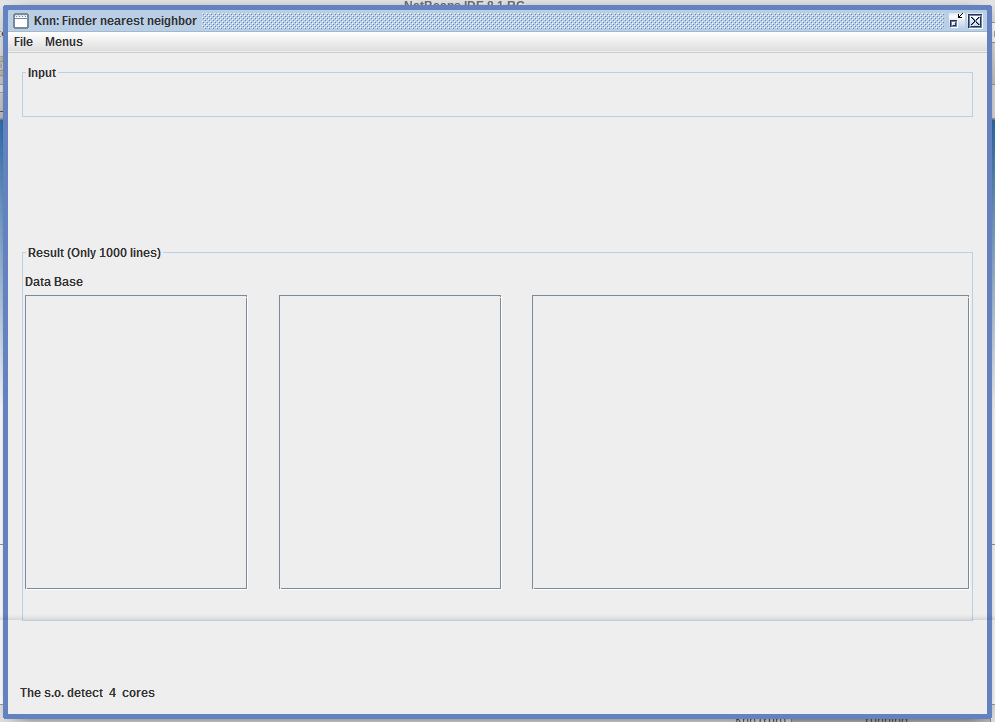
\includegraphics[width=14cm]{fig/interfaz1.png}
	\caption{\label{interfaz_inicial} Interfaz gráfica inicial del software}
\end{figure}      

\subsection*{Menús del software} \label{sec:menu}
El software posee dos menús como se menciono anteriormente, estos corresponden a $"File"$ y $"Menus"$, en el primer menú $File$ posee dos sub-menús $New$ y $Exit$, El primero posee sub-menús que corresponde a los algoritmos que posee el software, estos son:

\begin{itemize}
	\item \textit{Secuencial}
	\item \textit{Multihilos}
	\item \textit{Xeon Phi}
	\item \textit{GPU}
\end{itemize}

Cada uno de estos sub-menús, posee al menos un item que corresponde al algoritmo kNN programado de acuerdo a la lógica que su nombre indica, esto quiere decir que el sub-menú multihilos cuenta con a lo menos un item que permite ejecutar el algoritmo kNN multi-hilo, donde este utiliza \textit{OpenMP} para utilizar de mejor manera los recursos de la CPU.\\

Al seleccionar un item del sub-menú \textit{Multihilos} la interfaz gráfica tiene las siguientes características como se aprecia en la figura \ref{interfaz_multihilo}, en la sección $input$ se visualizan los campos de entrada que posee el software, en primer caso es la base de datos, esta se carga mediante el botón examinar, para cargar los datos de consulta se utiliza el botón examinar, $size obj$ es un valor numérico que corresponde a la magnitud del vector ingresado en la base de datos y base de consultas, $K$ es la cantidad de vecinos más cercanos que se desea obtener, $Threads$ por defecto se utiliza la cantidad cantidad de núcleos que posee la máquina donde esta instalado el software, este valor puede ser modificado por la cantidad de hilos que desea el usuario.\\
Además se cuenta con el botón $Start$ para comenzar a ejecutar el las consultas kNN, se añadió bajo el botón $Start$ un \textit{check box} que permite ejecutar un $Profiler$ que utiliza la librería PapiC \cite{iclit2017} que indica estadísticas sobre el uso de los hilos. En la sección $Result$ no varia en relación al item seleccionado.
 
\begin{figure}[hbtp]
	\centering
	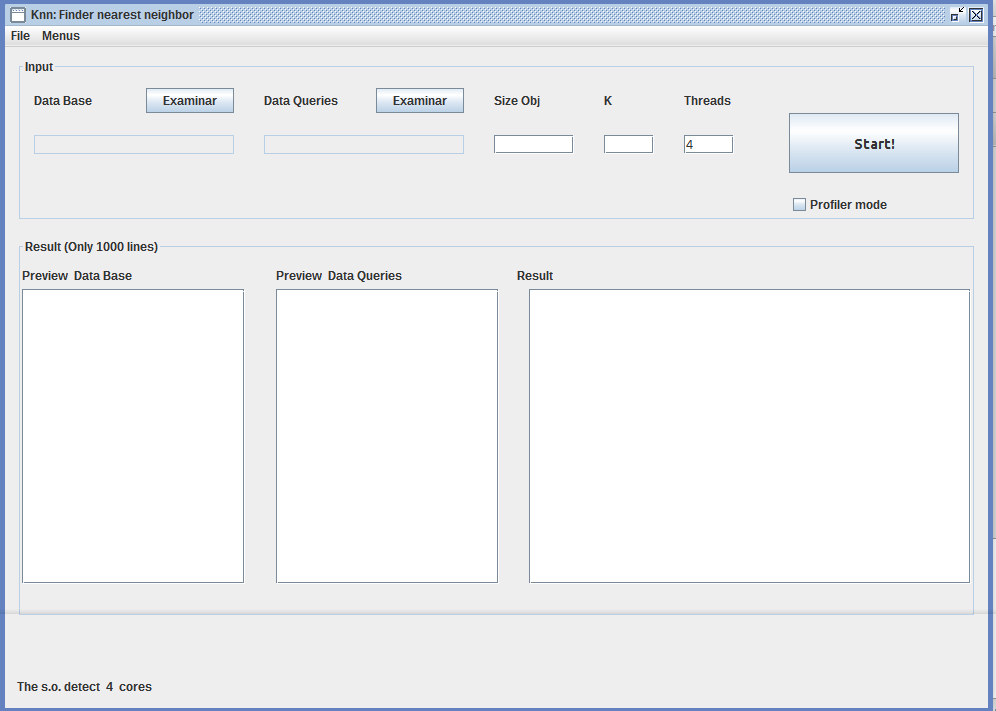
\includegraphics[width=14cm]{fig/interfaz_multicore}
	\caption{\label{interfaz_multihilo} Interfaz gráfica item multihilos del software}
\end{figure}
     
Al seleccionar un item del sub-menú \textit{Secuencial} la interfaz gráfica tiene las siguientes características como se aprecia en la figura \ref{interfaz_secuencial}, en la sección $input$ se visualizan los campos de entrada que posee el software, en primer caso es la base de datos, esta se carga mediante el botón examinar, para cargar los datos de consulta se utiliza el botón examinar, $size obj$ es un valor numérico que corresponde a la magnitud del vector ingresado en la base de datos y base de consultas, $K$ es la cantidad de vecinos más cercanos que se desea obtener.\\

\begin{figure}[hbtp]
	\centering
	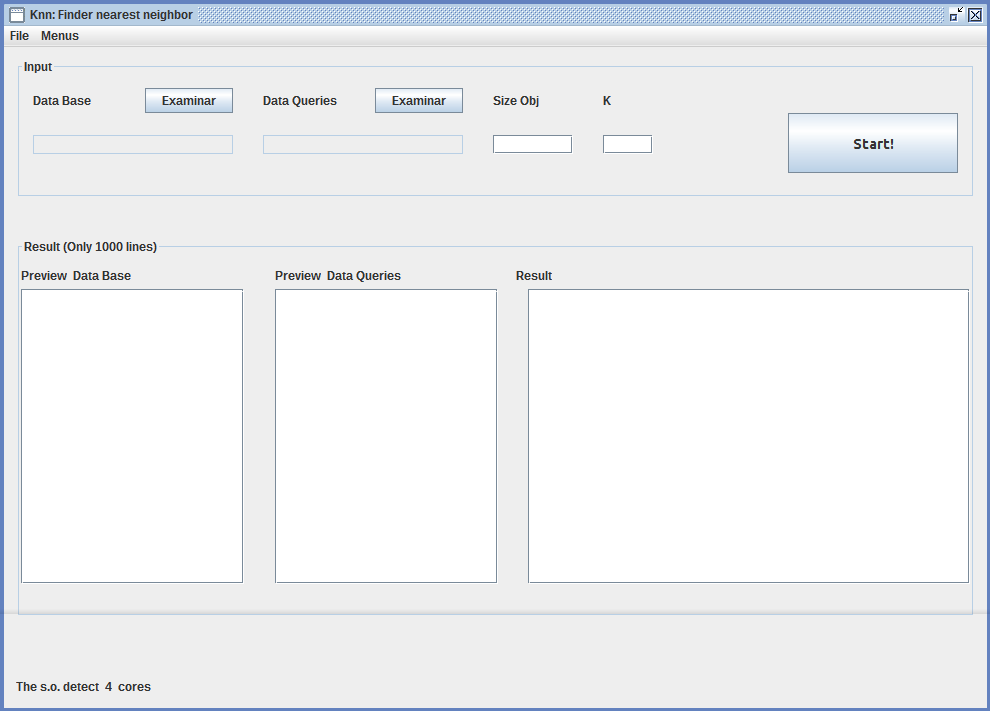
\includegraphics[width=14cm]{fig/interfaz_secuencial}
	\caption{\label{interfaz_secuencial} Interfaz gráfica item secuencial del software}
\end{figure}
 
La selección de los otros item en los sub-menús son similares a los antes mencionados, de modo que solamente varia la cantidad de datos de entrada que se ingresan dado las condiciones de programación de cada algoritmo.
\\\\
Además el software cuenta con mensajes dirigidos al usuario, estos son dividen en mensajes de alerta y mensajes de éxito. El primero se aprecia en la figura \ref{mensajes}\subref{fig:error}, este mensaje aparece una vez que se presiona el botón $Start$ y si algún campo está vacío, indica que campos debe completar para poder ejecutar correctamente el proceso. Si no presenta errores el proceso parte correctamente, si los archivos de bases de datos y consultas son archivos correspondientes, el proceso muestra un mensaje de éxito, como se aprecia en la figura \ref{mensajes}\subref{fig:exito}, al presionar el botón aceptar se muestra la ventana de los resultados de la consulta kNN, este paso corresponde a la sección \ref{sec:resultados} \textit{Métodos de exportación de resultados}.  

\begin{figure}
\begin{center}
\caption{\label{mensajes} Mensajes al usuario }
\subfigure[Mensaje 1 - Error]{
	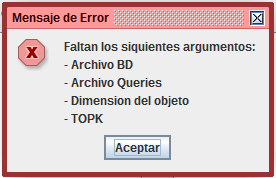
\includegraphics[width=5cm]{fig/error}
    \label{fig:error}
}~~~~~~~~~~~~
\subfigure[Mensaje 2 - Éxito]{
	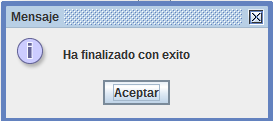
\includegraphics[width=5cm]{fig/exito_knn}
    \label{fig:exito}
}
\end{center}
\end{figure}

\section{Integración de algoritmo kNN Secuencial} \label{met:secuencial}

Si bien este algoritmo, no estaba considerado en un comienzo este se añadió para la posibilidad de poder ejecutar el software en equipos que no cuenten con procesadores con multi-núcleos y necesiten realizar consultas kNN. Este algoritmo se realizado con la estructura heap \ref{sec:heap}.\\
Para implementar el algoritmo kNN secuencial, se definió la estructura heap, la cual se aprecia en el segmento de código en el algoritmo \ref{lst:heap}, este almacena en $doble$ $dist$ la distancia del elemento consultado, ésta variable es de tipo $double$ debido a que las distancias son clasificadas como números reales y es posible obtener tener valores muy altos, a su vez $int ind$ indica la posición del vector dentro de la base de consultas. Cabe recalcar que solamente se almacenan K resultados en esta estructura, además de sólo almacenar los valores cuya distancia $dist$ sean las K menores.
\\ 
\begin{algorithm}
\begin{lstlisting}[language=C] 
struct _Elem {
    double dist;
    int ind;
};
typedef struct _Elem Elem;
\end{lstlisting}
\caption{\emph{\label{lst:heap}} Estructura para realizar los $Heap$.}
\end{algorithm}

Con el lenguaje de programación C, es posible utilizar la cantidad de memoria adecuada gracias a la instrucción $malloc$ que permite asignar la cantidad de memoria que corresponde al tamaño de la base de datos y al archivo de consulta. Esto último se aprecia en el algoritmo \ref{lst:malloc}, donde $consultas$ es una una matriz de $N\_queries x DIM$ donde $N\_queries$ es el número tuplas de vectores contenidas en la base de consulta y $DIM$ es el tamaño del vector. De manera análoga se establece la matriz $DB$ de $N\_DB x DIM$ donde $N\_DB$ es el número tuplas de vectores contenidas en la base de datos y $DIM$ es el tamaño del vector. A su vez $answer$ corresponde a la asignación de memoria para las $N\_queries$ con $K$ vecinos más cercanos donde se almacenan todas las respuestas a las consultas para ser finalmente mostrados. $Heap$ es la estructura a utilizar con cada consulta, esta corresponde a un heap del tipo heap max, donde el nodo padre es el mayor valor de la estructura.
\\
El desarrollo central del algoritmo para obtener los K vecinos más cercanos está dado por el algoritmo \ref{lst:knn}, este algoritmo indica las siguientes acciones, se establece un contador $n\_elem$ $=0$ que obtiene el número de elementos que han ingresado al heap, este se utiliza como comparador debido a que se deben ingresar K elementos al heap, mientras $n\_elem$ sea menor que el número $k$ se ingresaran los datos al heap en caso contrario se compara si la distancia del elemento actual es menor a la raíz del heap de manera que si el elemento es menor se extrae la raíz y se añade el elemento actual, y se reordena el heap. Este proceso itera exhaustivamente hasta que no queden elementos en la base de datos, cuando el heap está finalizado se almacenan sus resultados en la matriz $answer$ y se debe continuar con la siguiente consulta hasta que se procesen todas las consultas del base de consultas.

\begin{algorithm}
\begin{lstlisting}[language=C]
    Consultas = (double **) malloc(sizeof (double *)*N_QUERIES);
    for (i = 0; i < N_QUERIES; i++)
        Consultas[i] = (double *) malloc(sizeof (double)*DIM);

    DB = (double **) malloc(sizeof (double *)*N_DB);
    for (i = 0; i < N_DB; i++)
        DB[i] = (double *) malloc(sizeof (double)*DIM);

    answer = (Elem *)malloc(sizeof(Elem)*N_QUERIES*TOPK);
    
    heap = (Elem *) malloc(sizeof (Elem) * TOPK);
\end{lstlisting}
\caption{\emph{\label{lst:malloc}} Utilización de $malloc$.}
\end{algorithm}


\subsection{Funciones claves del algoritmo secuencial}  \label{met:claves}

$Distancia:$ Algoritmo \ref{lst:distancia} es la función de cálculo de la distancia entre vectores, tanto del vector de la base de datos y el vector de la base de consultas, este cálculo se realiza con la fórmula \eqref{ecu:distancia}.\\
Dados $A$ = $(X_1,Y_1)$ y $B$ = $(X_2,Y_2)$

\begin{equation}\label{ecu:distancia}
 distancia = \sqrt{(X_2-X_1)^{2}+(Y_2-Y_1)^{2}}
\end{equation}

Esta ecuación puede ser llevada a vectores de tamaño $n$.

\begin{algorithm}
\begin{lstlisting}[language=C]
double distancia(double *p1, double *p2) {
    int i = 0;
    double suma = 0;

    for (i = 0; i < DIM; i++)
        suma += ((p1[i] - p2[i])*(p1[i] - p2[i]));
    return sqrt(suma);
}  
\end{lstlisting}
\caption{\emph{\label{lst:distancia}} Cálculo de distancias entre vectores.}
\end{algorithm}


Sumado a esta función existen las funciones para manipular un heap, estas corresponden a obtener el valor nodo padre (Algoritmo \ref{lst:top}), realizar una inserción de un elemento, extraer un elemento y una añadida para facilitar el procedimiento del algoritmo cómo es el caso de una extracción e inserción que se utiliza cuando se debe cambiar un nodo dentro del heap y realizar el reordenamiento del heap.
\\
El algoritmo \ref{lst:top} retorna el valor de la raíz (nodo padre) del heap si no está vacío, en caso contrario retorna el valor máximo de un $double$.
   
\begin{algorithm}
\begin{lstlisting}[language=C]
double topH(Elem *heap, int *n_elem) {
    if (*n_elem == 0)
        return DBL_MAX;
    return heap[0].dist;
}
\end{lstlisting}
\caption{\emph{\label{lst:top}} Valor de la raíz del heap.}
\end{algorithm}

El algoritmo \ref{lst:inserta} realiza la inserción de un elemento, guardando la distancia y la posición del elemento, el contador $n\_elem$ incrementa en 1 luego de la inserción, y se realiza el ordenamiento del heap. Esta función es la que se utiliza en el algoritmo \ref{lst:heap} hasta llenar el heap.

\begin{algorithm}
\begin{lstlisting}[language=C]
void inserta(Elem *heap, Elem *elem, int *n_elem) {
    int i;
    Elem temp;

    heap[*n_elem].dist = elem->dist;
    heap[*n_elem].ind = elem->ind;
    (*n_elem)++;
    for (i = *n_elem; i > 1 && heap[i - 1].dist > heap[(i / 2) - 1].dist; i = i / 2) {
        temp = heap[i - 1];
        heap[i - 1] = heap[(i / 2) - 1];
        heap[(i / 2) - 1] = temp;
    }
}
\end{lstlisting}
\caption{\emph{\label{lst:inserta}} Realiza la inserción de un elemento al heap.}
\end{algorithm}

El algoritmo \ref{lst:extrae} realiza la extracción de un elemento, guardando la distancia y la posición del elemento, el contador $n\_elem$ decrementando en 1 luego de la extracción, y se realiza el ordenamiento del heap. Esta función es la que se utiliza para completar la matriz $answer$.

\begin{algorithm}
\begin{lstlisting}[language=C]
void extrae(Elem *heap, int *n_elem, Elem *elem_extraido) {
    int i, k;
    Elem temp;

    (*elem_extraido).dist = heap[0].dist;
    (*elem_extraido).ind = heap[0].ind;

    heap[0] = heap[(*n_elem) - 1]; // Movemos el ultimo a la raiz y achicamos el heap
    (*n_elem)--;
    i = 1;
    while (2 * i <= *n_elem) // mientras tenga algun hijo
    {
        k = 2 * i; //el hijo izquierdo
        if (k + 1 <= *n_elem && heap[(k + 1) - 1].dist > heap[k - 1].dist)
            k = k + 1; //el hijo derecho es el mayor
        if (heap[i - 1].dist > heap[k - 1].dist)
            break; //es mayor que ambos hijos

        temp = heap[i - 1];
        heap[i - 1] = heap[k - 1];
        heap[k - 1] = temp;
        i = k; //lo intercambiamos con el mayor hijo
    }
    return;
}
\end{lstlisting}
\caption{\emph{\label{lst:extrae}} Realiza la extracción de un elemento al heap.}
\end{algorithm}

El algoritmo \ref{lst:popush} realiza la extracción del elemento raíz y la posterior inserción del elemento cuya distancia era menor que la distancia del elemento raíz, esta función guarda la distancia y la posición del elemento, con esto luego se realiza el ordenamiento del heap. Esta función es la que se utiliza en el algoritmo \ref{lst:heap}  cuando el heap está lleno y se obtiene un elemento que cuya distancia es menor a la distancia de la raíz.


\begin{algorithm}
\begin{lstlisting}[language=C]

void popush(Elem *heap, int *n_elem, Elem *elem) {
    int i, k;
    Elem temp;

    heap[0].dist = elem->dist;
    heap[0].ind = elem->ind;

    i = 1;
    while (2 * i <= *n_elem) // mientras tenga algun hijo
    {
        k = 2 * i; //el hijo izquierdo
        if (k + 1 <= *n_elem && heap[(k + 1) - 1].dist > heap[k - 1].dist)
            k = k + 1; //el hijo derecho es el mayor
        if (heap[i - 1].dist > heap[k - 1].dist)
            break; //es mayor que ambos hijos

        temp = heap[i - 1];
        heap[i - 1] = heap[k - 1];
        heap[k - 1] = temp;
        i = k; //lo intercambiamos con el mayor hijo
    }
    return;
}

\end{lstlisting}
\caption{\emph{\label{lst:popush}} Realiza la extracción y la inserción de un elemento al heap.}
\end{algorithm}

Para realizar la integración de este algoritmo en la interfaz gráfica, se realizó mediante una rutina de $Java$ con $java.lang.Runtime.exec()$. La implementación de esta rutina permite ejecutar otro programa o ejecutable y luego obtener los resultados para ser visualizados a través de la interfaz gráfica creada en $Java$. El algoritmo \ref{lst:javarun} muestra un ejemplo simple de ejecutar un programa o ejecutable desde $Java$.

\begin{algorithm}
\begin{lstlisting}[language=Java]

import java.io.*;
 
public class llamarruntime
{
   public static void main(String[] args)
   {
      try{
         Process theProcess =
                 Runtime.getRuntime().exec(Ejecutable);
      }
      catch(IOException e){
         System.err.println("Error en el metodo exec()");
         e.printStackTrace();
      }
   } 
}
\end{lstlisting}
\caption{\emph{\label{lst:javarun}} Ejecutar un programa o ejecutable desde $Java$.}
\end{algorithm}


\section{Integración de la plataforma multi-núcleo} \label{sec:multi}


Este algoritmo posee ciertas semejanzas y diferencias con respecto a la versión secuencial, éste utiliza $malloc$ como se indica en el algoritmo \ref{lst:malloc}, estableciendo los mismos atributos y designando la memoria de la misma manera que la versión secuencial, léase \ref{met:secuencial}.
\\

La librería \textit{OpenMP} establece variables de tipo compartida \textit{Shared} y de tipo privadas \textit{Private}, donde con una variable del tipo compartida puede obtener su valor o realizar alguna modificación sin restricciones desde cualquier hilo. A su vez una variable del tipo privada solamente puede ser accesible por un hilo y crea una copia de la variable para tantos hilos creados existan. De esta manera se han establecido sólo variables del tipo \textit{Shared} para este algoritmo.

El desarrollo central del algoritmo para obtener los K vecinos más cercanos está dado por el algoritmo \ref{lst:knn2}, este algoritmo indica las siguientes acciones. Se establece un contador $n\_elem$ $=0$ que obtiene el número de elementos que han ingresado al heap, éste se utiliza como comparador debido a que se debe ingresar K elementos al heap, mientras $n\_elem$ sea menor que el número $K$ se ingresaran los datos al heap en caso contrario se compara si la distancia del elemento actual es menor a la raíz del heap de manera que si el elemento es menor, se extrae la raíz, se añade el elemento actual, y se reordena el heap. Este proceso itera paralelamente hasta que no queden elementos en la base de datos, cuando el heap está finalizado se almacenan sus resultados en la matriz $answer$ y se debe continuar con la siguiente consulta hasta que se procesen todas las consultas de la base de datos de consultas.



A diferencia del método secuencial, el método multi-hilo utiliza la librería OpenMP, por lo tanto como se muestra en el algoritmo \ref{lst:knn2} \textit{\#pragma omp master} indica el trabajo en la zona paralela, de manera que el ciclo $for$ realiza un paso cíclico con una cantidad determinada de hilos dada por $procs$, donde $tid$ es el identificador de cada hilo. Esto quiere decir que si se utiliza 2 hilos el hilo 0 con $tid=0$ realiza la consulta 0 y el hilo 1 con $tid=1$ realiza la consulta 1 simultáneamente finalizado el trabajo de al menos uno de éstos. El hilo con su actividad finalizada toma el valor correspondiente, en caso del hilo 0 con $tid=0$ le corresponde tomar la consulta 2 y al hilo 1 con $tid=1$ le corresponde el hilo 3. Este proceso se realiza hasta llegar al final de la base de datos de consultas $N\_queries$.\\

\subsection{Funciones claves del algoritmo multi-hilos}  

Estas funciones son las mismas que el método secuencial, donde se consideran $topH$ elementos para saber el valor del nodo raíz, $inserta$ para insertar un nodo en un heap con el número de elementos menor al de K elementos, $extrae$ extrae el nodo raíz del heap, $popush$ realiza la extracción del nodo raíz e inserción de un nuevo nodo de menor valor que la raíz extraída, léase \ref{met:claves}
\\
Para realizar la integración de este algoritmo en la interfaz gráfica se realizó mediante una rutina de $Java$ con $java.lang.Runtime.exec()$. La implementación de esta rutina permite ejecutar otro programa o ejecutable y obtener los resultados para ser visualizados a través de la interfaz gráfica creada en $Java$. El algoritmo \ref{lst:javarun} muestra un ejemplo simple de ejecutar un programa o ejecutable desde $Java$.
 

\section{Integración de algoritmo kNN Paralelo Xeon Phi}

A diferencia de los métodos anteriores acá se utiliza un coprocesador, de modo que se debe realizar la comunicación entre la CPU y el Coprocesador (\textit{Intel Xeon Phi}). A continuación se describe en detalle las funciones de este método.\\

Con el lenguaje de programación C, es posible utilizar la cantidad de memoria necesaria gracias a la instrucción $malloc$ que permite asignar la cantidad de memoria que corresponde al tamaño de la base de datos y la base de consulta, tal como se aprecia en el algoritmo \ref{lst:mallocxeon}. En este algoritmo $queries$ se crea una matriz de $num\_queries \times dimaux$ donde $num\_queries$ es el número tuplas de vectores contenidas en la base de consulta y $dimaux$ es el tamaño del vector. De manera análoga se establece la matriz $db$ de $num\_db \times dimaux$ donde $num\_db$ es el número tuplas de vectores contenidas en la base de datos y $dimaux$ es el tamaño del vector. A su vez $answer$ corresponde a la asignación de memoria para las $num\_queries$ con $K$ vecinos más cercanos donde se almacenan todas las respuestas a las consultas para ser finalmente mostrados. $Heap$ es la estructura a utilizar con cada consulta, ésta corresponde a un heap del tipo heap max, donde el nodo padre es el mayor valor de la estructura. La Xeon Phi sólo permite realizar el trabajo con vectores de modo que las matrices deben ser procesados como vectores y además los vectores deben ser múltiplos de 16, de modo que para solucionar este problema y poder trabajar con la medida de cualquier vector de entrada se parametriza a su vector múltiplo de 16 superior, en otras palabras si ingresa un vector de tamaño 8 se parametriza a 16, si ingresa un vector 17 se parametriza a 32 y los valores restantes son establecidos como 0, para no interferir en el cálculo de la distancia.  
\\
El desarrollo central del algoritmo para obtener los K vecinos más cercanos está dado por el algoritmo \ref{lst:knnxeon}, este algoritmo indica las siguientes acciones, las operaciones de este algoritmo están dentro de la región paralela de la Xeon Phi (\textit{\#pragma}) de manera que se debe enviar desde la CPU a la Xeon Phi todas las variables o constantes a utilizar, donde se deben cumplir ciertas restricciones como vectorizar la matriz (explicado anteriormente), además se especifican claramente cuales son datos exclusivamente de entrada \texttt{In} y exclusivamente datos de salida \texttt{Out} o datos que pueden ser de entrada y salida \texttt{(Inout)}. La Xeon Phi a través de la librería OpenMP utiliza además variables de tipo compartida y variables del tipo privadas, donde una variable del tipo compartida puede obtener su valor o realizar alguna modificación sin restricciones, a su vez una variable del tipo privada solamente puede ser accesible por un hilo y se crea una copia de la variable para tantos hilos creados existan. A diferencia del método anterior (Sección \ref{sec:multi}) que sólo utilizaba variables tipo compartida, en este método las variables del tipo privado se han establecido las siguientes variables \textit{i, j, thread\_num} de modo que cada hilo puede realizar independientemente sus iteraciones en los ciclos sin ser interrumpido por otro (línea 3 en Algoritmo \ref{lst:knnxeon}), esto debido a que se utilizan vectores y se debe emular la lectura de la matriz a través de los vectores. Dentro de la región paralela \textit{\#pragma omp parallel} se crea un heap de tamaño \textit{K}, luego se establece un contador $n\_elem$ $=0$ que obtiene el número de elementos que han ingresado al heap. Este último se utiliza como comparador debido a que se debe ingresar K elementos al heap, mientras $n\_elem$ sea menor que el número $k$ se ingresaran los datos al heap en caso contrario se compara si la distancia del elemento actual es menor a la raíz del heap, de manera que si el elemento es menor se extrae la raíz, se añade el elemento actual y se reordena el heap. Este proceso itera paralelamente hasta que no queden elementos en la base de datos y cuando el heap está finalizado se almacenan sus resultados en la matriz $answer$. Este proceso dentro de la región paralela \textit{\#pragma omp parallel} realiza cada uno de los pasos mencionados por cada hilo utilizado en el proceso\\



 \begin{algorithm}
\begin{lstlisting}[language=C]
   db= (double **)malloc(sizeof(double *)*num_db);
   for (i=0; i<num_db; i++)
      db[i] = (double *)malloc(sizeof(double)*dimaux);
   queries = (double **)malloc(sizeof(double *)*num_queries);
   for (i=0; i<num_queries; i++)
      queries[i] = (double *)malloc(sizeof(double)*dimaux);
   answer = (Elem *)malloc(sizeof(Elem)*num_queries*k);

   //Se transfieren datos de una matriz a un vector
   db_vector = (double *)_mm_malloc(sizeof(double)*dimaux*num_db, 64);
   for (i=0; i < dimaux*num_db; i++)
       db_vector[i] = 0.0;
   if (sizeof(double)*dimaux*num_queries < 64)
   {
        queries_vector = (double *)_mm_malloc(sizeof(double)*16, 64);
        for (i=0; i < 16; i++)
            queries_vector[i] = 0.0;
   }
   else
   {
        queries_vector = (double *)_mm_malloc(sizeof(double)*dimaux*num_queries, 64);
        for (i=0; i < dimaux*num_queries; i++)
            queries_vector[i] = 0.0;
   }
\end{lstlisting}
\caption{\emph{\label{lst:mallocxeon}}  Utilización de $malloc$.}
\end{algorithm}


\subsection{Funciones claves del algoritmo Xeon Phi}

A diferencia de los métodos anteriores donde solamente se utiliza una CPU, acá se emplea tanto la \textit{CPU} como un Coprocesador, el cual sólo realiza tareas específicas (léase \ref{cap:coprocesadores}). A continuación se detallan las principales funciones que se implementaron en \textit{Xeon Phi}.\\ 

$Distancia:$ Algoritmo \ref{lst:distanciaxeon} es la función de cálculo de la distancia entre vectores, tanto del vector de la base de datos y el vector de la base de consultas, este cálculo se realiza con la fórmula \eqref{ecu:distancia}. Esta función se realiza en la Xeon Phi para indicar que se realizaran en el coprocesador se utiliza la sintaxis \textit{\textbf{\_\_atribute\_\_((target(mic)))}}. Las sintaxis \textit{\textbf{\_\_assume\_aligned(), \#pragma vector aligned, \#pragma ivdep, \#pragma simd }} alinean los vectores y permiten que el cálculo de la distancia se realice correctamente.
  
\begin{algorithm}
\begin{lstlisting}[language=C]
__attribute__((target(mic))) double distancia(double *p1, double *p2, int DIM){
    int i=0;
    double suma=0.0;
   __assume_aligned(p1, 64);
   __assume_aligned(p2, 64);   
    #pragma vector aligned
    #pragma ivdep
    #pragma simd
    for (i=0; i < DIM; i++){
        suma += (p1[i]-p2[i])*(p1[i]-p2[i]);
    }
    return sqrt(suma);
}
\end{lstlisting}
\caption{\emph{\label{lst:distanciaxeon}} Función distancia \textit{Xeon Phi}.}
\end{algorithm}

Debido a que la \textit{Xeon Phi} no permite la utilización de matrices, se implementa la función \textit{matrixToVector} (Algoritmo \ref{lst:distanciaxeon}) para transferir la matriz a vector, esta función corresponde a la CPU no a la Xeon Phi de manera que no utiliza sintaxis especiales.

\begin{algorithm}
\begin{lstlisting}[language=C]
void matrixToVector(double **matrix, int num_cols, int num_rows, double *vector){
    int i,j;
    for(i=0; i<num_rows; i++)
        for(j=0; j<num_cols; j++)
            vector[(i*num_cols)+j] = matrix[i][j];
}
\end{lstlisting}
\caption{\emph{\label{lst:distanciaxeon}} Pasa una matriz a vector.}
\end{algorithm}

De manera similar a los métodos anteriores (Secuencial y Multi-núcleo) se emplean las mismas funciones, pero no se ejecutan en la CPU, éstas se ejecutan en el coprocesador- Para esto último, se añade al principio de cada función la sintaxis \textit{\textbf{\_\_atribute\_\_((target(mic)))}} por ejemplo el algoritmo \ref{lst:topxeon} que devuelve la raíz del heap, solamente varía en la sintaxis indicada anteriormente. A su vez tanto $inserta$, $extrae$, $popush$, se deben ejecutar en la Xeon Phi de modo que se debe añadir al principio de cada función la sintaxis \textit{\textbf{\_\_atribute\_\_((target(mic)))}}.\\\\

\begin{algorithm}
\begin{lstlisting}[language=C]
__attribute__((target(mic))) double topH(Elem *heap, int *n_elem)
{
    if ((*n_elem) == 0)
        return MAXDOUBLE;
    return heap[0].dist;
}
\end{lstlisting}
\caption{\emph{\label{lst:topxeon}} Valor de la raíz del heap.}
\end{algorithm}

Para realizar la integración de este algoritmo en la interfaz gráfica se realizó mediante una rutina de $Java$ con $java.lang.Runtime.exec()$. La implementación de esta rutina permite ejecutar otro programa o ejecutable, y obtener los resultados para ser visualizados a través de la interfaz gráfica creada en $Java$. El algoritmo \ref{lst:javarun} muestra un ejemplo simple de ejecutar un programa o ejecutable desde $Java$.
 


\section{Integración de algoritmo kNN Paralelo GPU}
Para GPU es necesario utilizar CUDA  (ver capitulo \ref{cap:cuda}), es una extensión de C, que permite la programación paralela que aprovecha la potencia de la GPU de NVIDIA, si bien la lógica central del algoritmo $kNN$ no varía de los métodos presentados anteriormente, sólo difiere en estructuras y/o sintaxis específicas de CUDA. De esta manera nos enfocaremos solamente en las funciones específicas utilizadas en este método.

Con el lenguaje de programación C, es posible utilizar la cantidad de memoria necesaria gracias a la instrucción $malloc$ que permite asignar la cantidad de memoria que corresponde al tamaño de la base de datos y la base de consulta, tal como se aprecia en el algoritmo \ref{lst:mallocCUDA}. En este algoritmo $Consultas$ se crea una matriz de $N\_Queries \times dimension$ donde $N\_QUERIES$ es el número tuplas de vectores contenidas en la base de consulta y $dimension$ es el tamaño del vector. De manera análoga se establece la matriz $vectores$ de $N\_ELEM \times dimension$ donde $N\_ELEM$ es el número tuplas de vectores contenidas en la base de datos y $dimension$ es el tamaño del vector. A su vez $res\_final\_H$ (línea 8 algoritmo \ref{lst:knncuda}) corresponde a la asignación de memoria para las $N\_Queries$ con $K$ vecinos más cercanos donde se almacenan todas las respuestas a las consultas para ser finalmente mostrados. $Linea\_temp$  (línea 8 algoritmo \ref{lst:knncuda}) es la estructura a utilizar con cada consulta, esta corresponde a un heap max, donde el nodo raíz es el mayor valor de la estructura, considerar que la lectura de las consultas se realiza de modo inverso a la lectura de las bases de datos.

Como se aprecia en el algoritmo \ref{lst:knnCUDA}, se utiliza la función $Batch\_Heap\_Reduction$ con $N\_BLOQUES$ que indica la cantidad de bloques a utilizar y $T\_per\_BLOCK$ que indica la cantidad de hilos por bloques.\\ 
El algoritmo \ref{lst:bacth} realiza todo el proceso de cada una de las consultas, donde cada bloque realiza una consulta con los $T\_per\_BLOCK$ hilos por bloque. De manera que realiza la evaluación de la consulta y se almacenan en el Heap las primeras K, finalizado esto se realiza la evaluación con el nodo raíz del heap, si el elemento actual es menor que el elemento del nodo, se reemplaza sino se mantiene el heap de la misma manera. 


\begin{algorithm}
\begin{lstlisting}[language=C]
  res_final_H = (double *)malloc(sizeof(double)*Q*TOPK);
  
  Elem *linea_temp = (Elem *)malloc(sizeof(Elem)*Q*T_per_BLOCK);
  
  
  consultas =(double **)malloc(sizeof(double *)*N_QUERIES);
  for (i=0; i<N_QUERIES; i++)
    consultas[i] = (double *)malloc(sizeof(double)*dimension);
    
  vectores =(double **)malloc(sizeof(double *)*dimension);
  for (i=0; i<dimension; i++)
    vectores[i] = (double *)malloc(sizeof(double)*N_ELEM);
  
\end{lstlisting}
\caption{\emph{\label{lst:mallocCUDA}} Utilización de $malloc$.}
\end{algorithm}

\subsection{Funciones claves del algoritmo GPU NVIDIA}

De manera diferente de los métodos secuenciales y multi-hilos donde solamente se utiliza una CPU, acá se emplea tanto la CPU como un coprocesador el cual sólo realiza tareas específicas (léase \ref{cap:coprocesadores}). A continuación se detallan las principales funciones que se implementaron en GPU NVDIA.\\ 

Si bien la lógica principal del algoritmo kNN no varía, si lo hacen las instrucciones para ser implementadas como se ha observado en los distintos métodos, y el caso de la GPU no es diferente, ya que ésta cuenta con su propia librería de CUDA y difiere de acuerdo a cada nueva versión de la arquitectura que está diseñada la GPU. Cada función que es implementada en GPU tiene como inicio de la declaración de la función $\_\_device\_\_$. 

A continuación se describen las principales funciones en GPU, donde el algoritmo \ref{lst:insertagpu} se encarga de realizar la inserción de los elementos en un heap. Éste a diferencia de los anteriores difiere en la forma de su sintaxis dado particularmente en la forma de acceder a cierta posición del heap, debido a la forma en que NVIDIA realiza el acceso a este tipo de estructuras. El algoritmo \ref{lst:extraegpu} realiza la extracción de la raíz del heap y lo reordena como corresponde. A su vez en algoritmo \ref{lst:distanciaGPU} si el heap está lleno, realiza la extracción de la raíz del heap e, inserta el nuevo elemento y reorganiza el heap. A su vez el algoritmo \ref{lst:distanciaGPU} calcula  la distancia euclidiana pero con la matriz de consultas transversa debido que el acceso de esta manera en GPU permite ser aun más rápido en ejecución.    


\begin{algorithm}
\begin{lstlisting}[language=C]

__device__ void insertaH(Elem *heap, Elem *elem, int *n_elem, int pitch, int id){
  int i;
  Elem temp;

  ((Elem *)((char *)heap + (*n_elem)*pitch))[id].dist = elem->dist;
  ((Elem *)((char *)heap + (*n_elem)*pitch))[id].ind = elem->ind;
  (*n_elem)++;
  
  for (i = *n_elem; i>1 && ((Elem *)((char *)heap + (i-1)*pitch))[id].dist > ((Elem *)((char *)heap + ((i/2)-1)*pitch))[id].dist; i=i/2){
    //Intercambiamos con el padre
    temp.dist = ((Elem *)((char *)heap + (i-1)*pitch))[id].dist;
    temp.ind = ((Elem *)((char *)heap + (i-1)*pitch))[id].ind;
    ((Elem *)((char *)heap + (i-1)*pitch))[id].dist = ((Elem *)((char *)heap + ((i/2)-1)*pitch))[id].dist;
    ((Elem *)((char *)heap + (i-1)*pitch))[id].ind = ((Elem *)((char *)heap + ((i/2)-1)*pitch))[id].ind;
    ((Elem *)((char *)heap + ((i/2)-1)*pitch))[id].dist = temp.dist;
    ((Elem *)((char *)heap + ((i/2)-1)*pitch))[id].ind = temp.ind;
  }
  return;
}
  
\end{lstlisting}
\caption{\emph{\label{lst:insertagpu}} Inserta un elemento en el heap.}
\end{algorithm}

Para realizar la integración de este algoritmo en la interfaz gráfica se realizó mediante una rutina de $Java$ con $java.lang.Runtime.exec()$. La implementación de esta rutina permite ejecutar otro programa o ejecutable y obtener los resultados para ser visualizados a través de la interfaz gráfica creada en $Java$. (Algoritmo \ref{lst:javarun}).


\begin{algorithm}
\begin{lstlisting}[language=C]

__device__ void extraeH(Elem *heap, int *n_elem, int pitch, int id, Elem *eresult){
  
  int i, k;
  Elem temp;
  eresult->dist = ((Elem *)((char *)heap+0))[id].dist; //Se guarda el maximo
  eresult->ind = ((Elem *)((char *)heap+0))[id].ind; 

  ((Elem *)((char *)heap+0))[id].dist = ((Elem *)((char *)heap + ((*n_elem)-1)*pitch))[id].dist;// Movemos el ultimo a la raiz y achicamos el heap
  ((Elem *)((char *)heap+0))[id].ind = ((Elem *)((char *)heap + ((*n_elem)-1)*pitch))[id].ind;
  (*n_elem)--;
  i = 1;
  while(2*i <= *n_elem)
  {
    k = 2*i; //el hijo izquierdo
    if(k+1 <= *n_elem && ((Elem *)((char *)heap + ((k+1)-1)*pitch))[id].dist > ((Elem *)((char *)heap + (k-1)*pitch))[id].dist)
      k = k+1;

    if(((Elem *)((char *)heap + (i-1)*pitch))[id].dist > ((Elem *)((char *)heap + (k-1)*pitch))[id].dist)
      break;

    temp.dist = ((Elem *)((char *)heap + (i-1)*pitch))[id].dist;
    temp.ind = ((Elem *)((char *)heap + (i-1)*pitch))[id].ind;
    ((Elem *)((char *)heap + (i-1)*pitch))[id].dist = ((Elem *)((char *)heap + (k-1)*pitch))[id].dist;
    ((Elem *)((char *)heap + (i-1)*pitch))[id].ind = ((Elem *)((char *)heap + (k-1)*pitch))[id].ind;
    ((Elem *)((char *)heap + (k-1)*pitch))[id].dist = temp.dist;
    ((Elem *)((char *)heap + (k-1)*pitch))[id].ind = temp.ind;
    i = k;   //lo intercambiamos con el mayor hijo
  }
  return;
}
  
\end{lstlisting}
\caption{\emph{\label{lst:extraegpu}} Realiza la extracción de un elemento del $heap$}
\end{algorithm}

\begin{algorithm}
\begin{lstlisting}[language=C]

__device__ double topH(Elem *heap, int id){
  return ((Elem *)((char *)heap + 0))[id].dist;
}
  
\end{lstlisting}
\caption{\emph{\label{lst:mallocCUDA}} Obtener el valor de la raíz del $heap$}
\end{algorithm}

\begin{algorithm}
\begin{lstlisting}[language=C]

__device__ void popush(Elem *heap, Elem *elem, int *n_elem, int pitch, int id){

  int i, k;
  Elem temp;

  ((Elem *)((char *)heap+0))[id].dist = elem->dist;
  ((Elem *)((char *)heap+0))[id].ind  = elem->ind;

  i = 1;
  while(2*i <= *n_elem) // mientras tenga algun hijo
  {
    k = 2*i; //el hijo izquierdo
    if(k+1 <= *n_elem && ((Elem *)((char *)heap + ((k+1)-1)*pitch))[id].dist > ((Elem *)((char *)heap + (k-1)*pitch))[id].dist)
      k = k+1;  //el hijo derecho es el mayor

    if(((Elem *)((char *)heap + (i-1)*pitch))[id].dist > ((Elem *)((char *)heap + (k-1)*pitch))[id].dist)
      break;  //es mayor que ambos hijos

    temp.dist = ((Elem *)((char *)heap + (i-1)*pitch))[id].dist;
    temp.ind = ((Elem *)((char *)heap + (i-1)*pitch))[id].ind;
    ((Elem *)((char *)heap + (i-1)*pitch))[id].dist = ((Elem *)((char *)heap + (k-1)*pitch))[id].dist;
    ((Elem *)((char *)heap + (i-1)*pitch))[id].ind = ((Elem *)((char *)heap + (k-1)*pitch))[id].ind;
    ((Elem *)((char *)heap + (k-1)*pitch))[id].dist = temp.dist;
    ((Elem *)((char *)heap + (k-1)*pitch))[id].ind = temp.ind;
    i = k;   //lo intercambiamos con el mayor hijo
  }
  return;
}
  
\end{lstlisting}
\caption{\emph{\label{lst:popushgpu}} Realiza la extracción y la inserción de un elemento al $heap$}
\end{algorithm}

\begin{algorithm}
\begin{lstlisting}[language=C]

__device__ double distancia_trans(double *p1, int pitch_p1, int col_1, double *q){

   int i=0;
   double suma=0;

   for (i=0; i < DIM; i++)
      suma += (((double *)((char *)p1 + (i*pitch_p1)))[col_1] - q[i]) * 
              (((double *)((char *)p1 + (i*pitch_p1)))[col_1] - q[i]);

   return sqrtf(suma);  
}
  
\end{lstlisting}
\caption{\emph{\label{lst:distanciaGPU}} Cálculo de distancia con matriz transpuesta}
\end{algorithm}


\section{Métodos de exportación de resultados}\label{sec:resultados}

La exportación de los resultados obtenidos se realiza en consideración de los formatos más utilizados comúnmente, como son archivos de texto plano (.txt), formato de documento portable (.pdf), archivos Word (.doc), archivos de hojas de cálculo (.xls), La figura \ref{exportar} muestra como es la interfaz gráfica de esta parte del software.\\\\

Como se mencionó en la sección anterior \ref{sec:menu}, cuando se ejecuta exitosamente un algoritmo kNN se muestra la ventana gráfica de los resultados obtenidos, en la parte central de la figura \ref{exportar} se aprecia el recuadro donde se muestran todos los resultados de los K vecinos más cercanos de cada uno de las consultas realizadas.
\\

\begin{figure}[hbtp]
	\centering
	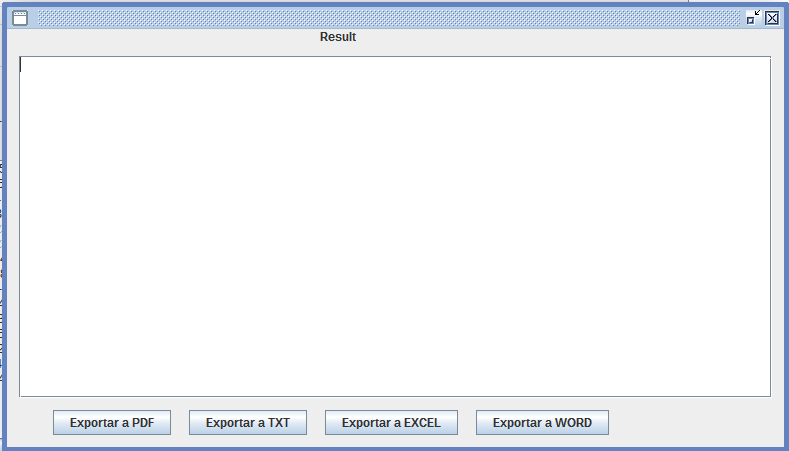
\includegraphics[width=14cm]{fig/resultados}
	\caption{\label{exportar} Interfaz gráfica de ventana de exportación de resultados}
\end{figure}

\begin{figure}[hbtp]
	\centering
	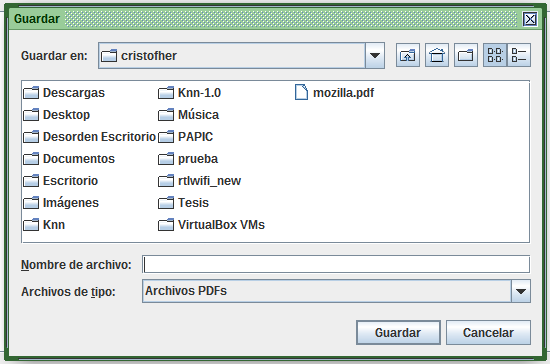
\includegraphics[width=10cm]{fig/guardar}
	\caption{\label{guardar} Interfaz gráfica de ventana de guardar archivo}
\end{figure}


En la figura \ref{guardar} se muestra la gráfica de la opción guardar. Cuando se selecciona cualquiera de los tipos de exportación, la gráfica es la misma y es intuitiva de acuerdo al común de las gráficas de exportación de diversos software.
\\
En los algoritmos (\ref{lst:excel},\ref{lst:pdf},\ref{lst:txt})  se muestra extracto de los códigos de exportación de acuerdo con sus formatos, el primer método (Algoritmo \ref{lst:excel}) corresponde al método de exportación de resultados a Excel en formato $.xls$. Para implementar tanto la exportación a Word y a Excel fue necesario incluir una API llamada $POI$ en su \textit{versión 3.16} \cite{poi}, esta API permite que desde una aplicación desarrollada en $Java$ se pueda exportar a diversos formatos como \textit{Word, Hojas de cálculo, Presentaciones, etc.} siendo los dos primeros considerados en esta tesis.
\\
El segundo método (Algoritmo \ref{lst:pdf}) es el caso de la exportación a Formato de documento portátil $(PDF)$, y para ello fue necesario la importación de $iText$ en su \textit{versión 5} \cite{itex}, siendo esta biblioteca de código libre (Open Source) desarrollada por iText Group, y está disponible para $Java$ y $C\#$. Esta API permite crear y manipular archivos \textit{PDF - RTF - HTML} en java, siendo el primero considerado para esta tesis. 
\\
El tercer método (Algoritmo \ref{lst:txt}) es el caso de la exportación a archivo de texto plano $(TXT)$, para este tipo de documentos no se utilizó librerías externas debido a que $Java$ posee métodos para la creación y manipulación de estos archivos.   
\\
Los métodos mencionados anteriormente cuentan con una función $obtenerRutaArchivo$, esta permite guardar el archivo con el nombre que le da el usuario y la extensión correspondiente al documento que desea exportar. En caso que el archivo que desea crear ya existe pide la confirmación al usuario si se debe reemplazar el archivo.

\noindent
\begin{algorithm}
\begin{lstlisting}[language=Java] 
public void generarExcel() throws IOException {
    String rutaArchivo = obtenerRutaArchivo("xls", "Archivos Excel");
    if (rutaArchivo != null && jTextArea1.getText().length() != 0) {
        File archivoXLS = new File(rutaArchivo);
        if (archivoXLS.exists()) {
            archivoXLS.delete();
        }
        archivoXLS.createNewFile();
        Workbook libro = new HSSFWorkbook();
        FileOutputStream archivo = new FileOutputStream(archivoXLS);
        Sheet hoja = (Sheet) libro.createSheet("Resultados Knn");
        String texto = jTextArea1.getText();
        String[] lineas = texto.split("\n");
        for (int i = 0; i < lineas.length; i++) {
            Row fila = hoja.createRow(i);
            String[] sublineas = lineas[i].split(" ");
            for (int j = 0; j < sublineas.length; j++) {
                 Cell celda = fila.createCell(j);
                 celda.setCellValue(sublineas[j]);
             }
         }
         libro.write(archivo);
         archivo.close();
         }
}
\end{lstlisting}
\caption{\emph{\label{lst:excel}} Método de exportación de resultados a $Excel$.}
\end{algorithm}

\begin{algorithm}
\begin{lstlisting}[language=Java] 
public void generarPDF() throws IOException, DocumentException {
        String rutaArchivo = obtenerRutaArchivo("pdf", "Archivos PDFs");
        if (rutaArchivo != null) {
            File archivoPDF = new File(rutaArchivo);
            if (archivoPDF.exists()) {
                archivoPDF.delete();
            }
            archivoPDF.createNewFile();
            FileOutputStream archivo = new FileOutputStream(archivoPDF);
            Document documento = new Document();
            PdfWriter.getInstance(documento, archivo);
            documento.open();
            documento.add(new Paragraph("Resultados Knn \n"));
            String texto = jTextArea1.getText();
            String[] lineas = texto.split("\n");
            for (String linea : lineas) {
                documento.add(new Paragraph(linea));
            }
            documento.close();
            JOptionPane.showMessageDialog(null,
                    "El archivo se a guardado Exitosamente",
                    "Informacion", JOptionPane.INFORMATION_MESSAGE);
        }
    }
\end{lstlisting}
\caption{\emph{\label{lst:pdf}} Método de exportación de resultados a $PDF$.}
\end{algorithm}

\begin{algorithm}
\begin{lstlisting}[language=Java] 
    public void generarTXT() throws IOException {
        String rutaArchivo = obtenerRutaArchivo("txt", "Archivo de texto plano TXT");
        try {
            if (rutaArchivo != null) {
                File archivoTXT = new File(rutaArchivo);
                if (archivoTXT.exists()) {
                    archivoTXT.delete();
                }
                try (FileWriter save = new FileWriter(archivoTXT)) {
                    save.write(jTextArea1.getText());
                }
                JOptionPane.showMessageDialog(null,
                        "El archivo se a guardado Exitosamente",
                        "Informacion", JOptionPane.INFORMATION_MESSAGE);
                Desktop.getDesktop().open(archivoTXT);
            }
        } catch (IOException ex) {
            JOptionPane.showMessageDialog(null,
                    "Su archivo no se ha guardado",
                    "Advertencia", JOptionPane.WARNING_MESSAGE);
        }

    }
\end{lstlisting}
\caption{\emph{\label{lst:txt}} Método de exportación de resultados a $TXT$.}
\end{algorithm}

  
\section{Nuevo módulo: Añadir menú} 

Para añadir un nuevo método al software además de los que ya cuenta por defecto, el usuario cuenta con un menú de opciones para añadir un método creado por él, pero debe cumplir con ciertos requisitos estipulados de acuerdo con cada uno de los tipos de algoritmo ya sea secuencial o paralelo según la arquitectura.
\\
Cabe mencionar que la realización de este menú, fue realizado a través de una interfaz gráfica en JAVA y su lógica en el lenguaje C, de manera que se dividen las tareas en base al principio divide y vencerás. La interfaz gráfica como se aprecia en la figura \ref{exportar}, donde se aprecia en la parte izquierda de la interfaz los 4 tipos de algoritmos contenidos en el software de modo que si desea ingresar un nuevo algoritmo. Se debe indicar a cual de ellos pertenece, de manera similar a la carga de bases de datos y consultas se debe cargar el archivo fuente, este será visto previamente en el recuadro inferior izquierdo. Además del paso anterior debe especificar el nombre del menú el cual aparecerá en la lista de los menús. Para finalizar y lograr añadir correctamente un nuevo método debe presionar el botón \textit{Compile \& add Menu} y el recuadro inferior derecho mostrara información detallada respecto del proceso de compilación, de manera que indica si el proceso fue exitoso o no.  

\begin{figure}[hbtp]
	\centering
	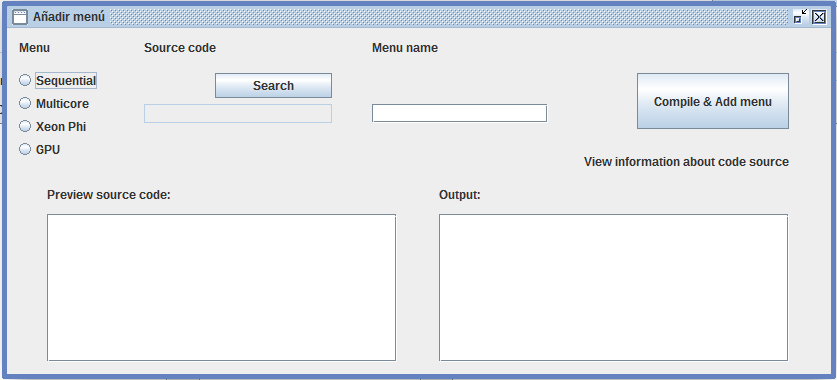
\includegraphics[width=15cm]{fig/add_menu.png}
	\caption{\label{exportar} Interfaz gráfica de ventana Agregar menú}
	\end{figure}
